\section{error control instead of defect control}
Another idea is to consider error control instead of defect control for the continuous approximate solution. We would thus need a way to create two interpolants, one of a higher order and one of a lower order and sample the difference between these two interpolants to estimate the error of the continuous solution approximation. 
=== A step-size selection algorithm based on that error estimate could provide an effective error controlled solution.

An issue with defect control is the V-shape of the defect. 
We know that this is entirely because of the $\frac{1}{h}$ in the derivative definition of the Hermite-Birkhoff interpolants as the interpolant itself does not suffer from round-off error but its derivative does.

\subsection{error is not v-shaped}
For all the schemes, the defect is V-shaped but the error itself is not. 
This is because the Hermite-Birkhoff interpolant does not contain a term in $\frac{1}{h}$ whereas its derivative does contain such a term. 
Figure $\ref{fig:defect_is_v_shape}$ and $\ref{fig:error_is_not_v_shape}$ shows this phenomenon for HB6 but the same can be see for HB4 and HB8. 

\begin{figure}[H]
\centering
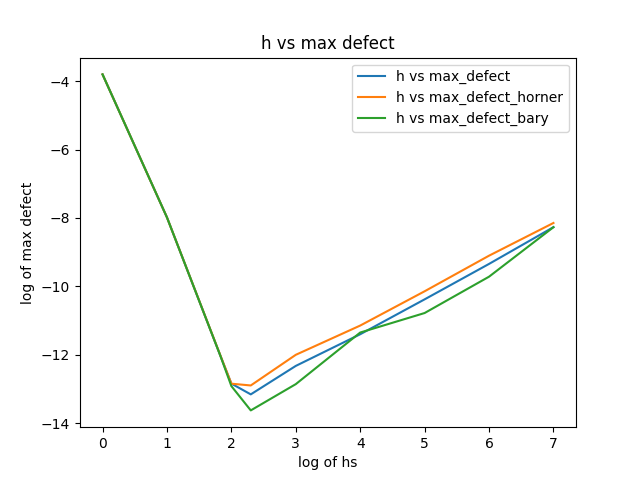
\includegraphics[width=0.7\linewidth]{./figures/further_work_defect_is_v_shape_hb6}
\caption{Defect has V-shape.}
\label{fig:defect_is_v_shape}
\end{figure}

\begin{figure}[H]
\centering
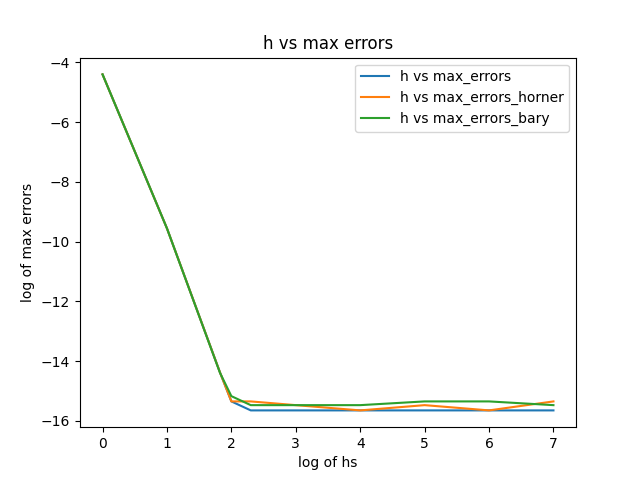
\includegraphics[width=0.7\linewidth]{./figures/further_work_error_is_not_v_shape_hb6}
\caption{Error does not have V-shape.}
\label{fig:error_is_not_v_shape}
\end{figure}

we sample
\begin{equation}
| h(x) - l(x) |
\end{equation}
at two x values within $x_i$ and $x_{i+1}$ and take the max to get the error estimate within the step.

\subsection{rk4 with hb4 vs hb6 with sampling}
Because we do not differentiate and that hb4 has order 4, we can use with rk4 with HB4 for error control. Thus HB4 and HB6 should not suffer from much interpolation error and we can use rk4 with the hb4 and hb6 using the error scheme

\paragraph{Problem 1} Figures $\ref{fig:rk4_with_hb4_hb6_sampling_p1_global_error}$ and $\ref{fig:rk4_with_hb4_hb6_sampling_p1_scaled_errors}$ shows the global error and the shape of the error on each step of using rk4 with hb4 vs hb6 with sampling on Problem 1 at an absolute tolerance of $10^{-6}$. From Figure $\ref{fig:rk4_with_hb4_hb6_sampling_p1_scaled_errors}$, we can see that there is no consistent location where the exact error between the returned interpolant and the exact solution can be sampled. However, internally, the solver uses an estimated error between the two interpolants that it uses. In Figure $\ref{fig:rk4_with_hb4_hb6_sampling_p1_scaled_estimated_errors}$, we can see that the maximum error occurs reasonably consistently at $0.5h$.

\begin{figure}[H]
\centering
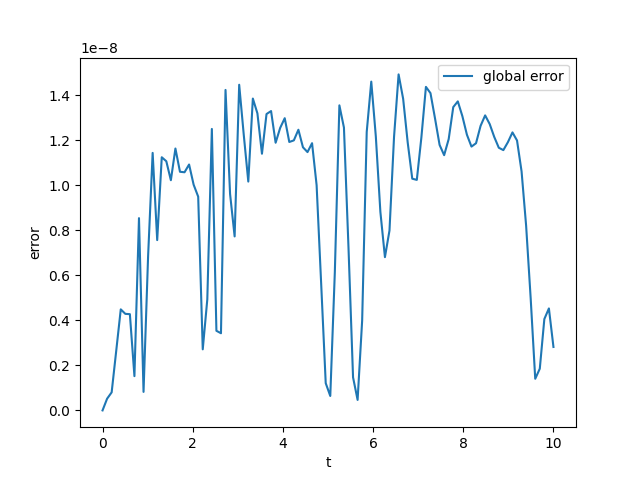
\includegraphics[width=0.7\linewidth]{./figures/rk4_with_hb4_hb6_sampling_p1_global_error}
\caption{Global Error for RK4 with HB4 vs HB6 with error sampling on problem 1 at an absolute tolerance of $10^{-6}$.}
\label{fig:rk4_with_hb4_hb6_sampling_p1_global_error}
\end{figure}

\begin{figure}[H]
\centering
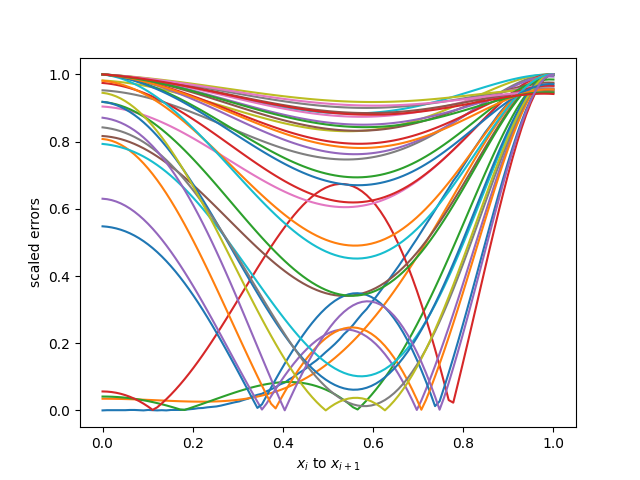
\includegraphics[width=0.7\linewidth]{./figures/rk4_with_hb4_hb6_sampling_p1_scaled_errors}
\caption{Scaled exact errors over all steps for RK4 with HB4 vs HB6 with error sampling on problem 1 at an absolute tolerance of $10^{-6}$ mapped onto $[0, 1]$.}
\label{fig:rk4_with_hb4_hb6_sampling_p1_scaled_errors}
\end{figure}

\begin{figure}[H]
\centering
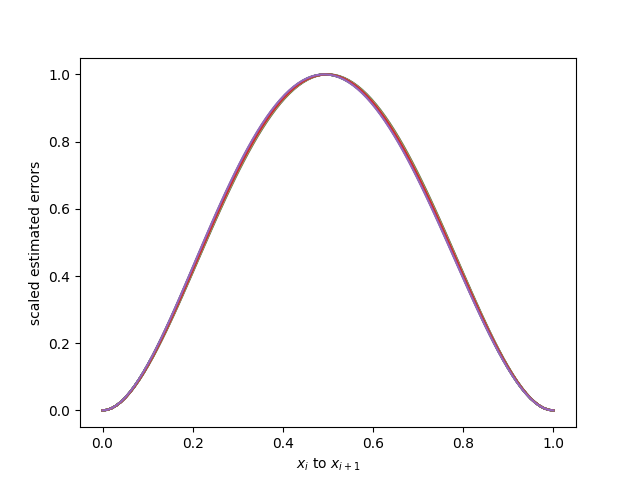
\includegraphics[width=0.7\linewidth]{./figures/rk4_with_hb4_hb6_sampling_p1_scaled_estimated_errors}
\caption{Scaled estimated errors over all steps for RK4 with HB4 vs HB6 with error sampling on problem 1 at an absolute tolerance of $10^{-6}$ mapped onto $[0, 1]$.}
\label{fig:rk4_with_hb4_hb6_sampling_p1_scaled_estimated_errors}
\end{figure}

\paragraph{Problem 2} Figures $\ref{fig:rk4_with_hb4_hb6_sampling_p2_global_error}$ and $\ref{fig:rk4_with_hb4_hb6_sampling_p2_scaled_errors}$ shows the global error and the shape of the error on each step of using rk4 with hb4 vs hb6 with sampling on Problem 2 at an absolute tolerance of $10^{-6}$. From Figure $\ref{fig:rk4_with_hb4_hb6_sampling_p2_scaled_errors}$, we can see that there is no consistent location where the exact error between the returned interpolant and the exact solution can be sampled. However, internally, the solver uses an estimated error between the two interpolants that it uses. In Figure $\ref{fig:rk4_with_hb4_hb6_sampling_p2_scaled_estimated_errors}$, we can see that the maximum error occurs reasonably consistently at $0.5h$.

\begin{figure}[H]
\centering
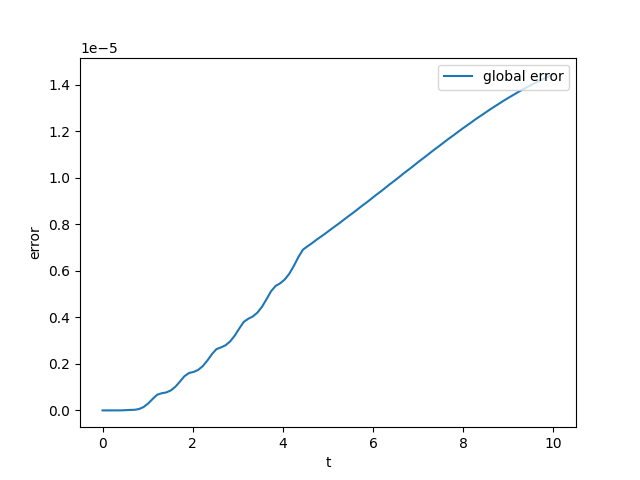
\includegraphics[width=0.7\linewidth]{./figures/rk4_with_hb4_hb6_sampling_p2_global_error}
\caption{Global Error for RK4 with HB4 vs HB6 with error sampling on problem 2 at an absolute tolerance of $10^{-6}$.}
\label{fig:rk4_with_hb4_hb6_sampling_p2_global_error}
\end{figure}

\begin{figure}[H]
\centering
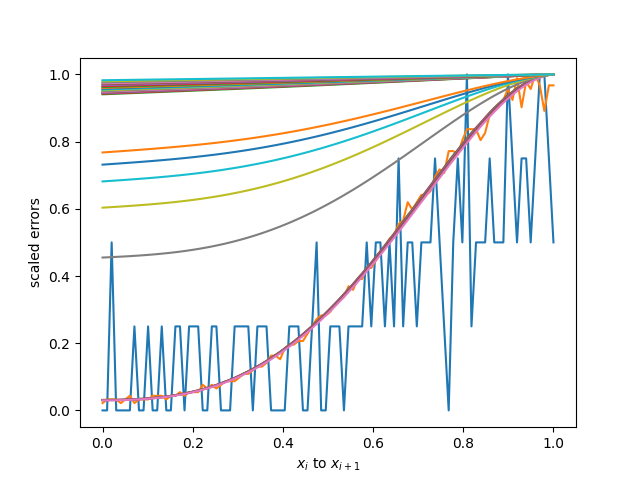
\includegraphics[width=0.7\linewidth]{./figures/rk4_with_hb4_hb6_sampling_p2_scaled_errors}
\caption{Scaled exact errors over all steps for RK4 with HB4 vs HB6 with error sampling on problem 2 at an absolute tolerance of $10^{-6}$ mapped onto $[0, 1]$.}
\label{fig:rk4_with_hb4_hb6_sampling_p2_scaled_errors}
\end{figure}

\begin{figure}[H]
\centering
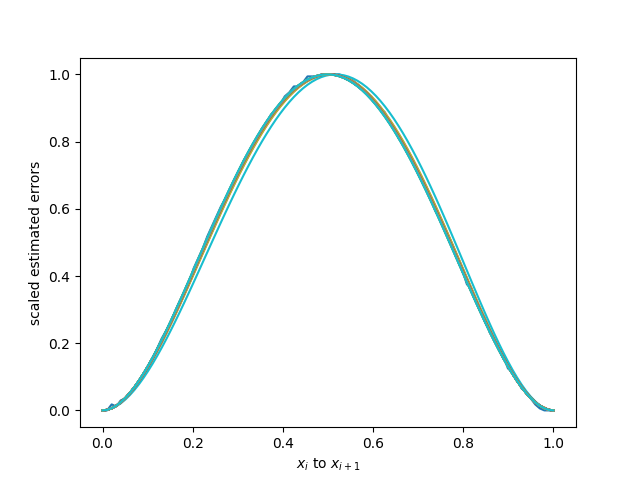
\includegraphics[width=0.7\linewidth]{./figures/rk4_with_hb4_hb6_sampling_p2_scaled_estimated_errors}
\caption{Scaled estimated errors over all steps for RK4 with HB4 vs HB6 with error sampling on problem 2 at an absolute tolerance of $10^{-6}$ mapped onto $[0, 1]$.}
\label{fig:rk4_with_hb4_hb6_sampling_p2_scaled_estimated_errors}
\end{figure}


\paragraph{Problem 3} Figures $\ref{fig:rk4_with_hb4_hb6_sampling_p3_global_error}$ and $\ref{fig:rk4_with_hb4_hb6_sampling_p3_scaled_errors}$ shows the global error and the shape of the error on each step of using rk4 with hb4 vs hb6 with sampling on Problem 3 at an absolute tolerance of $10^{-6}$. From Figure $\ref{fig:rk4_with_hb4_hb6_sampling_p3_scaled_errors}$, we can see that there is no consistent location where the exact error between the returned interpolant and the exact solution can be sampled. However, internally, the solver uses an estimated error between the two interpolants that it uses. In Figure $\ref{fig:rk4_with_hb4_hb6_sampling_p3_scaled_estimated_errors}$, we can see that the maximum error occurs reasonably consistently at $0.5h$

\begin{figure}[H]
\centering
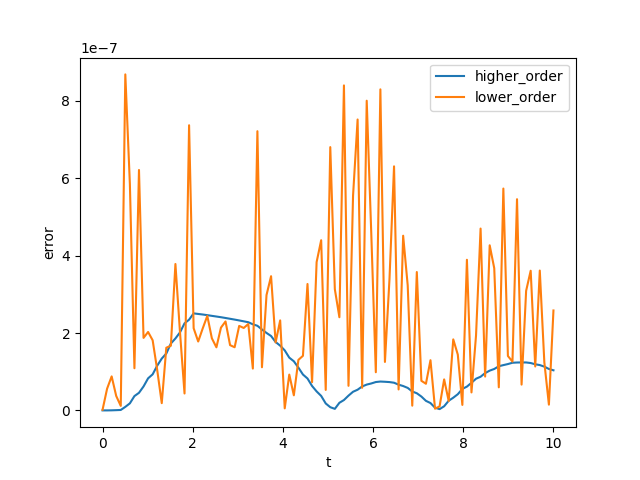
\includegraphics[width=0.7\linewidth]{./figures/rk4_with_hb4_hb6_sampling_p3_global_error}
\caption{Global Error for RK4 with HB4 vs HB6 with error sampling on problem 3 at an absolute tolerance of $10^{-6}$.}
\label{fig:rk4_with_hb4_hb6_sampling_p3_global_error}
\end{figure}

\begin{figure}[H]
\centering
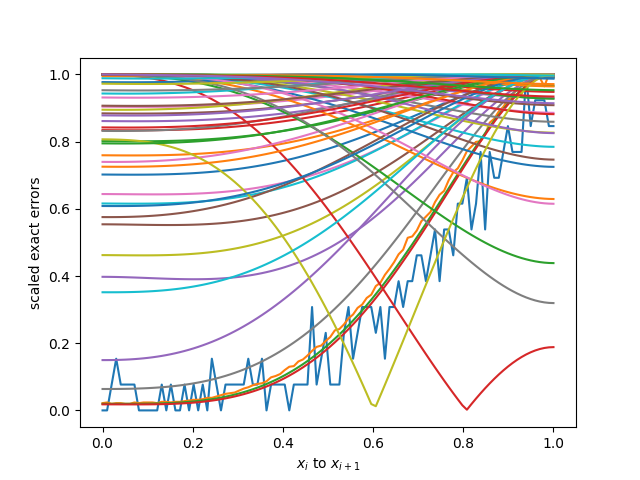
\includegraphics[width=0.7\linewidth]{./figures/rk4_with_hb4_hb6_sampling_p3_scaled_errors}
\caption{Scaled exact errors over all steps for RK4 with HB4 vs HB6 with error sampling on problem 3 at an absolute tolerance of $10^{-6}$ mapped onto $[0, 1]$.}
\label{fig:rk4_with_hb4_hb6_sampling_p3_scaled_errors}
\end{figure}

\begin{figure}[H]
\centering
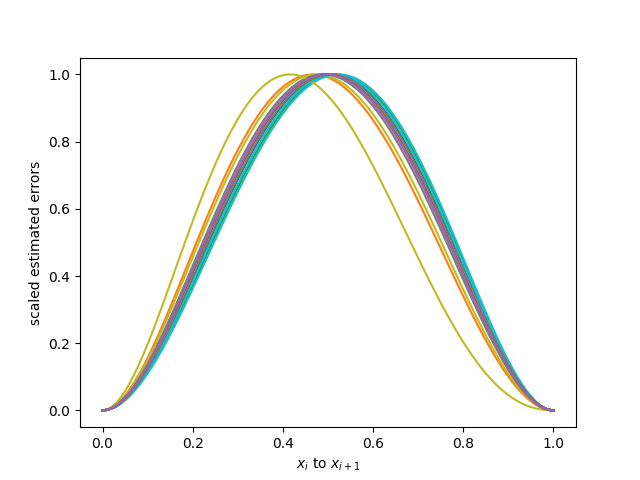
\includegraphics[width=0.7\linewidth]{./figures/rk4_with_hb4_hb6_sampling_p3_scaled_estimated_errors}
\caption{Scaled estimated errors over all steps for RK4 with HB4 vs HB6 with error sampling on problem 3 at an absolute tolerance of $10^{-6}$ mapped onto $[0, 1]$.}
\label{fig:rk4_with_hb4_hb6_sampling_p3_scaled_estimated_errors}
\end{figure}


\begin{table}[h]
\caption {Number of steps taken by RK4 using error control with HB4 vs HB6 by sampling the error.} \label{tab:rk4_with_hb4_hb6_sampling_nsteps}
\begin{center}
\begin{tabular}{ c c c } 
Problem & successful steps & total steps \\ 
1       & 35                         & 37 \\ 
2       & 30                         & 34 \\
3       & 75                         & 97 \\
\end{tabular}
\end{center}
\end{table}


\subsubsection{rk4 with hb4 vs hb8}
can be considered
\subsubsection{rk4 with hb4 vs hb10}
can be considered
\subsubsection{rk4 with hb6 vs hb8}
can be considered
\subsubsection{rk4 with hb6 vs hb10}
can be considered
\subsubsection{rk4 with hb8 vs hb10}
can be considered

\subsection{rk6 with hb6 vs hb8 with sampling}
Because we do not differentiate and that hb6 has order 6, we can use with rk6 with HB6 for error control. Thus HB6 and HB8 should not suffer from much interpolation error and we can use rk6 with the hb4 and hb6 using the error scheme

\paragraph{Problem 1} Figures $\ref{fig:rk6_with_hb6_hb8_sampling_p1_global_error}$ and $\ref{fig:rk6_with_hb6_hb8_sampling_p1_scaled_errors}$ shows the global error and the shape of the error on each step of using rk6 with hb6 vs hb8 with sampling on Problem 1 at an absolute tolerance of $10^{-6}$. From Figure $\ref{fig:rk6_with_hb6_hb8_sampling_p1_scaled_errors}$, we can see that there is no consistent location where the exact error between the returned interpolant and the exact solution can be sampled. However, internally, the solver uses an estimated error between the two interpolants that it uses. In Figure $\ref{fig:rk6_with_hb6_hb8_sampling_p1_scaled_estimated_errors}$, we can see that the maximum error occurs reasonably consistently at $0.5h$.

\begin{figure}[H]
\centering
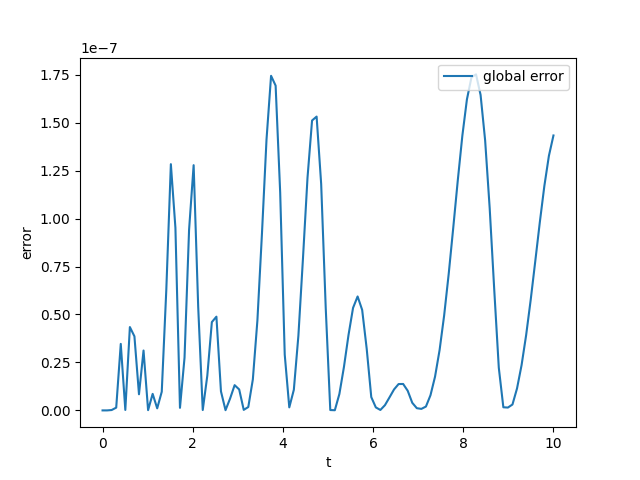
\includegraphics[width=0.7\linewidth]{./figures/rk6_with_hb6_hb8_sampling_p1_global_error}
\caption{Global Error for RK6 with HB6 vs HB8 with error sampling on problem 1 at an absolute tolerance of $10^{-6}$.}
\label{fig:rk6_with_hb6_hb8_sampling_p1_global_error}
\end{figure}

\begin{figure}[H]
\centering
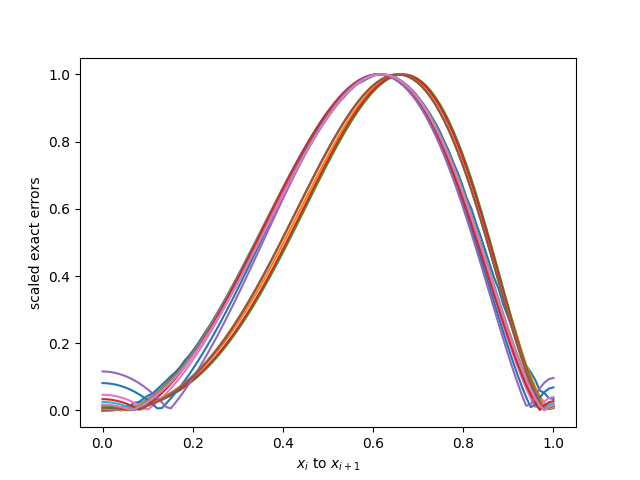
\includegraphics[width=0.7\linewidth]{./figures/rk6_with_hb6_hb8_sampling_p1_scaled_errors}
\caption{Scaled exact errors over all steps for RK6 with HB6 vs HB8 with error sampling on problem 1 at an absolute tolerance of $10^{-6}$ mapped onto $[0, 1]$.}
\label{fig:rk6_with_hb6_hb8_sampling_p1_scaled_errors}
\end{figure}

\begin{figure}[H]
\centering
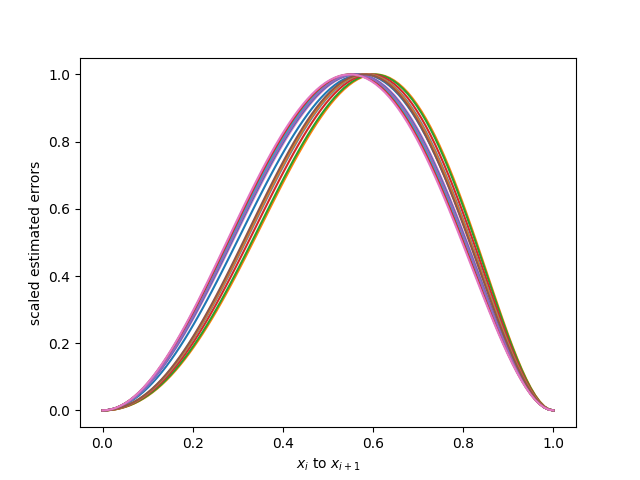
\includegraphics[width=0.7\linewidth]{./figures/rk6_with_hb6_hb8_sampling_p1_scaled_estimated_errors}
\caption{Scaled estimated errors over all steps for RK6 with HB6 vs HB8 with error sampling on problem 1 at an absolute tolerance of $10^{-6}$ mapped onto $[0, 1]$.}
\label{fig:rk6_with_hb6_hb8_sampling_p1_scaled_estimated_errors}
\end{figure}


\paragraph{Problem 2} Figures $\ref{fig:rk6_with_hb6_hb8_sampling_p2_global_error}$ and $\ref{fig:rk6_with_hb6_hb8_sampling_p2_scaled_errors}$ shows the global error and the shape of the error on each step of using rk6 with hb6 vs hb8 with sampling on Problem 2 at an absolute tolerance of $10^{-6}$. From Figure $\ref{fig:rk6_with_hb6_hb8_sampling_p2_scaled_errors}$, we can see that there is no consistent location where the exact error between the returned interpolant and the exact solution can be sampled. However, internally, the solver uses an estimated error between the two interpolants that it uses. In Figure $\ref{fig:rk6_with_hb6_hb8_sampling_p2_scaled_estimated_errors}$, we can see that the maximum error occurs reasonably consistently at $0.5h$.

\begin{figure}[H]
\centering
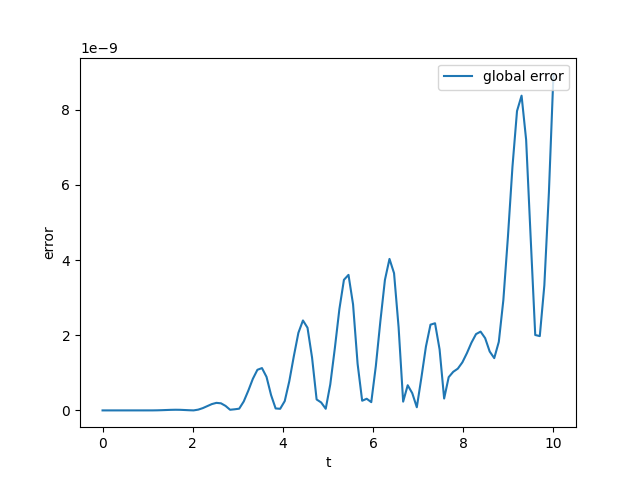
\includegraphics[width=0.7\linewidth]{./figures/rk6_with_hb6_hb8_sampling_p2_global_error}
\caption{Global Error for RK6 with HB6 vs HB8 with error sampling on problem 2 at an absolute tolerance of $10^{-6}$.}
\label{fig:rk6_with_hb6_hb8_sampling_p2_global_error}
\end{figure}

\begin{figure}[H]
\centering
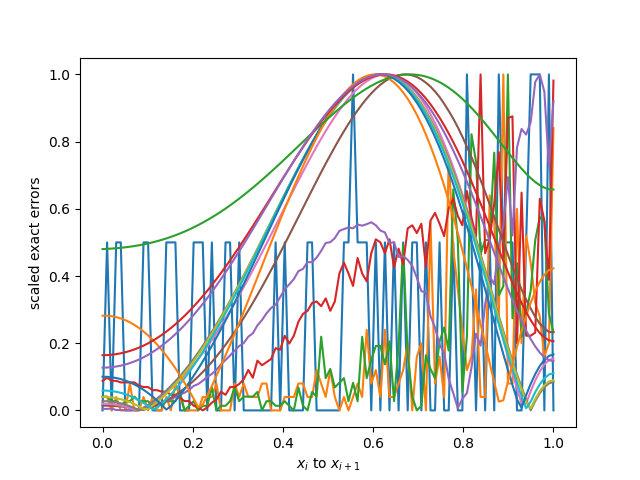
\includegraphics[width=0.7\linewidth]{./figures/rk6_with_hb6_hb8_sampling_p2_scaled_errors}
\caption{Scaled exact errors over all steps for RK6 with HB6 vs HB8 with error sampling on problem 2 at an absolute tolerance of $10^{-6}$ mapped onto $[0, 1]$.}
\label{fig:rk6_with_hb6_hb8_sampling_p2_scaled_errors}
\end{figure}

\begin{figure}[H]
\centering
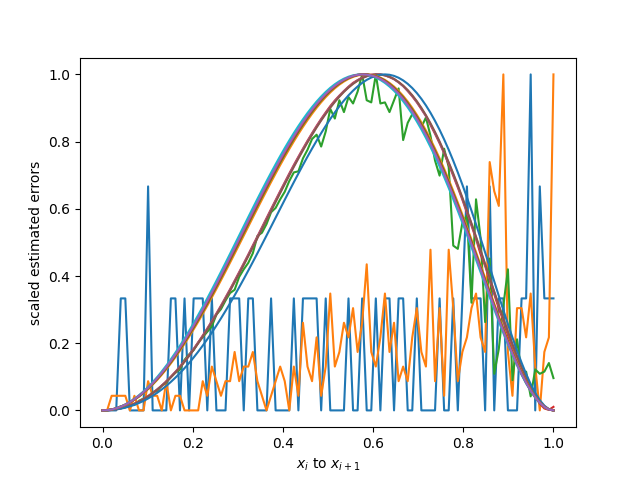
\includegraphics[width=0.7\linewidth]{./figures/rk6_with_hb6_hb8_sampling_p2_scaled_estimated_errors}
\caption{Scaled estimated errors over all steps for RK6 with HB6 vs HB8 with error sampling on problem 2 at an absolute tolerance of $10^{-6}$ mapped onto $[0, 1]$.}
\label{fig:rk6_with_hb6_hb8_sampling_p2_scaled_estimated_errors}
\end{figure}

\paragraph{Problem 3} Figures $\ref{fig:rk6_with_hb6_hb8_sampling_p3_global_error}$ and $\ref{fig:rk6_with_hb6_hb8_sampling_p3_scaled_errors}$ shows the global error and the shape of the error on each step of using rk6 with hb6 vs hb8 with sampling on Problem 3 at an absolute tolerance of $10^{-6}$. From Figure $\ref{fig:rk6_with_hb6_hb8_sampling_p3_scaled_errors}$, we can see that there is no consistent location where the exact error between the returned interpolant and the exact solution can be sampled. However, internally, the solver uses an estimated error between the two interpolants that it uses. In Figure $\ref{fig:rk6_with_hb6_hb8_sampling_p3_scaled_estimated_errors}$, we can see that the maximum error occurs reasonably consistently at $0.5h$.

\begin{figure}[H]
\centering
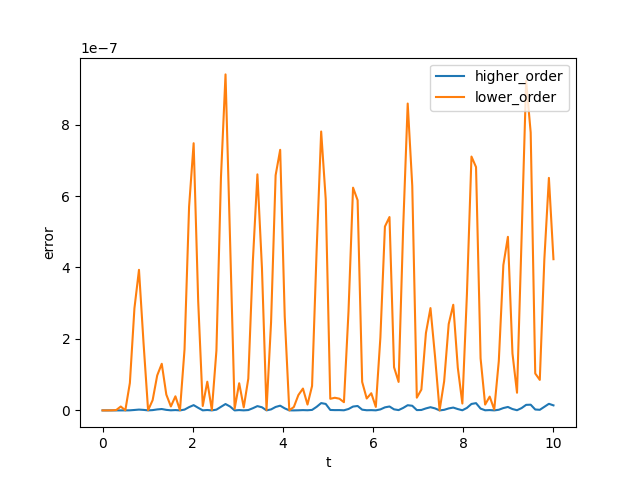
\includegraphics[width=0.7\linewidth]{./figures/rk6_with_hb6_hb8_sampling_p3_global_error}
\caption{Global Error for RK6 with HB6 vs HB8 with error sampling on problem 3 at an absolute tolerance of $10^{-6}$.}
\label{fig:rk6_with_hb6_hb8_sampling_p3_global_error}
\end{figure}

\begin{figure}[H]
\centering
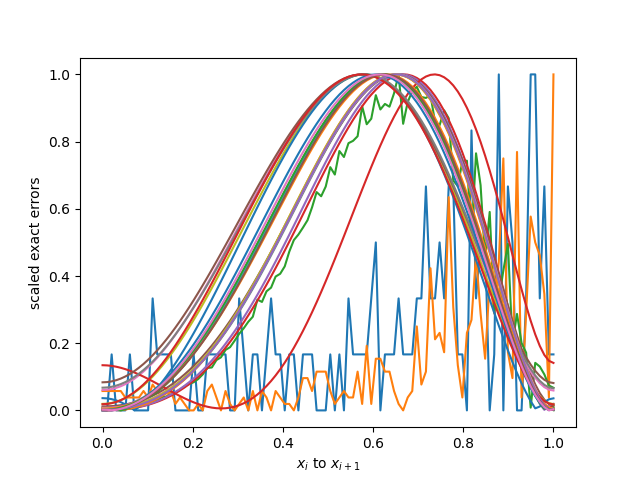
\includegraphics[width=0.7\linewidth]{./figures/rk6_with_hb6_hb8_sampling_p3_scaled_errors}
\caption{Scaled exact errors over all steps for RK6 with HB6 vs HB8 with error sampling on problem 3 at an absolute tolerance of $10^{-6}$ mapped onto $[0, 1]$.}
\label{fig:rk6_with_hb6_hb8_sampling_p3_scaled_errors}
\end{figure}

\begin{figure}[H]
\centering
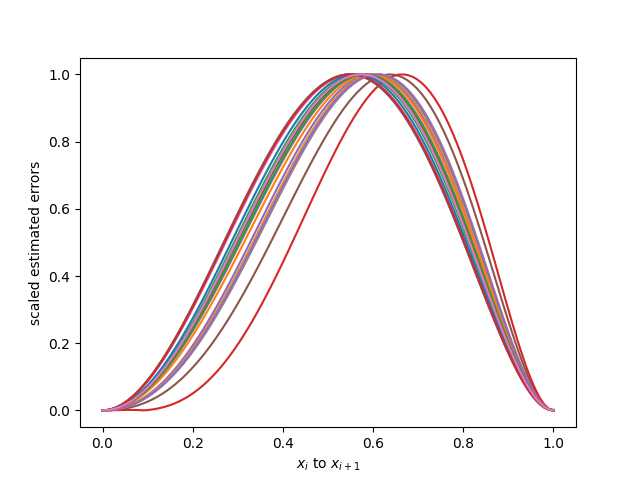
\includegraphics[width=0.7\linewidth]{./figures/rk6_with_hb6_hb8_sampling_p3_scaled_estimated_errors}
\caption{Scaled estimated errors over all steps for RK6 with HB6 vs HB8 with error sampling on problem 3 at an absolute tolerance of $10^{-6}$ mapped onto $[0, 1]$.}
\label{fig:rk6_with_hb6_hb8_sampling_p3_scaled_estimated_errors}
\end{figure}

\begin{table}[h]
\caption {Number of steps taken by RK6 using error control with HB6 vs HB8 by sampling the error.} \label{tab:rk6_with_hb6_hb8_sampling_nsteps}
\begin{center}
\begin{tabular}{ c c c } 
Problem & successful steps & total steps \\ 
1       & 17                         & 17 \\ 
2       & 15                         & 21 \\
3       & 27                         & 34 \\
\end{tabular}
\end{center}
\end{table}

\subsubsection{rk6 with hb6 vs hb10}
can be considered
\subsubsection{rk6 with hb8 vs hb10}
can be considered

\subsection{rk8 with hb8 vs hb10}
Because we do not differentiate and that hb8 has order 8, we can use with rk8 with HB8 for error control. Thus HB8 and HB10 should not suffer from much interpolation error and we can use rk8 with the hb8 and hb10 using the error scheme

\paragraph{Problem 1} Figures $\ref{fig:rk8_with_hb8_hb10_sampling_p1_global_error}$ and $\ref{fig:rk8_with_hb8_hb10_sampling_p1_scaled_errors}$ shows the global error and the shape of the error on each step of using rk8 with hb8 vs hb10 with sampling on Problem 1 at an absolute tolerance of $10^{-6}$. From Figure $\ref{fig:rk8_with_hb8_hb10_sampling_p1_scaled_errors}$, we can see that there is no consistent location where the exact error between the returned interpolant and the exact solution can be sampled. However, internally, the solver uses an estimated error between the two interpolants that it uses. In Figure $\ref{fig:rk8_with_hb8_hb10_sampling_p1_scaled_estimated_errors}$, we can see that the maximum error occurs reasonably consistently at $0.6h$.

\begin{figure}[H]
\centering
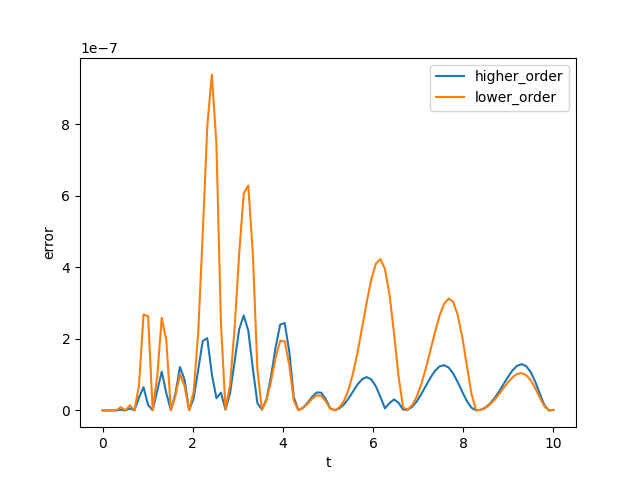
\includegraphics[width=0.7\linewidth]{./figures/rk8_with_hb8_hb10_sampling_p1_global_error}
\caption{Global Error for RK8 with HB8 vs HB10 with error sampling on problem 1 at an absolute tolerance of $10^{-6}$.}
\label{fig:rk8_with_hb8_hb10_sampling_p1_global_error}
\end{figure}

\begin{figure}[H]
\centering
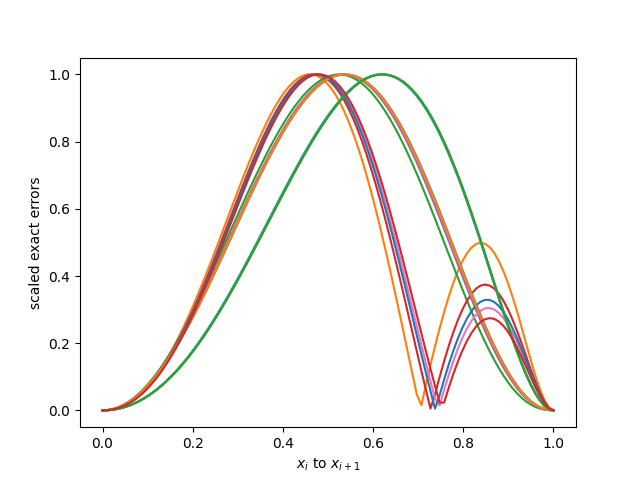
\includegraphics[width=0.7\linewidth]{./figures/rk8_with_hb8_hb10_sampling_p1_scaled_errors}
\caption{Scaled exact errors over all steps for RK8 with HB8 vs HB10 with error sampling on problem 1 at an absolute tolerance of $10^{-6}$ mapped onto $[0, 1]$.}
\label{fig:rk8_with_hb8_hb10_sampling_p1_scaled_errors}
\end{figure}

\begin{figure}[H]
\centering
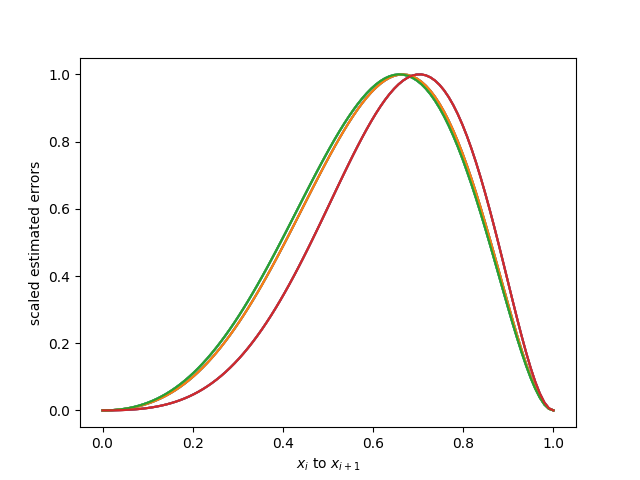
\includegraphics[width=0.7\linewidth]{./figures/rk8_with_hb8_hb10_sampling_p1_scaled_estimated_errors}
\caption{Scaled estimated errors over all steps for RK8 with HB8 vs HB10 with error sampling on problem 1 at an absolute tolerance of $10^{-6}$ mapped onto $[0, 1]$.}
\label{fig:rk8_with_hb8_hb10_sampling_p1_scaled_estimated_errors}
\end{figure}


\paragraph{Problem 2} Figures $\ref{fig:rk8_with_hb8_hb10_sampling_p2_global_error}$ and $\ref{fig:rk8_with_hb8_hb10_sampling_p2_scaled_errors}$ shows the global error and the shape of the error on each step of using rk8 with hb8 vs hb10 with sampling on Problem 2 at an absolute tolerance of $10^{-6}$. From Figure $\ref{fig:rk8_with_hb8_hb10_sampling_p2_scaled_errors}$, we can see that there is no consistent location where the exact error between the returned interpolant and the exact solution can be sampled. However, internally, the solver uses an estimated error between the two interpolants that it uses. In Figure $\ref{fig:rk8_with_hb8_hb10_sampling_p2_scaled_estimated_errors}$, we can see that the maximum error occurs reasonably consistently at $0.6h$.

\begin{figure}[H]
\centering
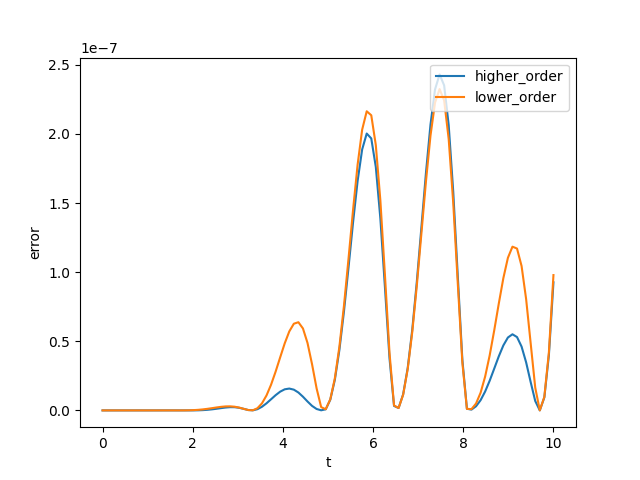
\includegraphics[width=0.7\linewidth]{./figures/rk8_with_hb8_hb10_sampling_p2_global_error}
\caption{Global Error for RK8 with HB8 vs HB10 with error sampling on problem 2 at an absolute tolerance of $10^{-6}$.}
\label{fig:rk8_with_hb8_hb10_sampling_p2_global_error}
\end{figure}

\begin{figure}[H]
\centering
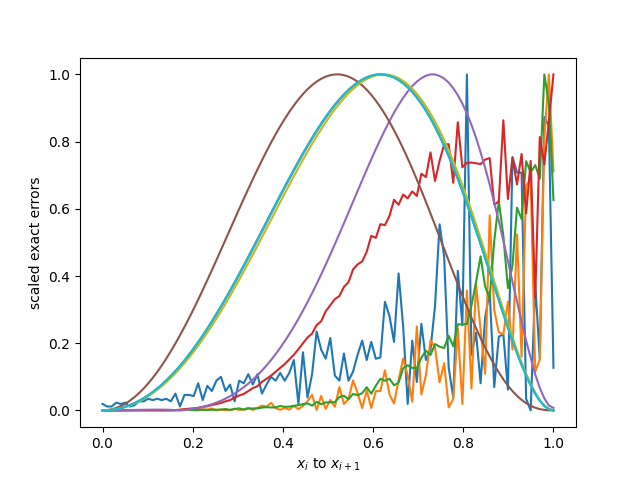
\includegraphics[width=0.7\linewidth]{./figures/rk8_with_hb8_hb10_sampling_p2_scaled_errors}
\caption{Scaled exact errors over all steps for RK8 with HB8 vs HB10 with error sampling on problem 2 at an absolute tolerance of $10^{-6}$ mapped onto $[0, 1]$.}
\label{fig:rk8_with_hb8_hb10_sampling_p2_scaled_errors}
\end{figure}

\begin{figure}[H]
\centering
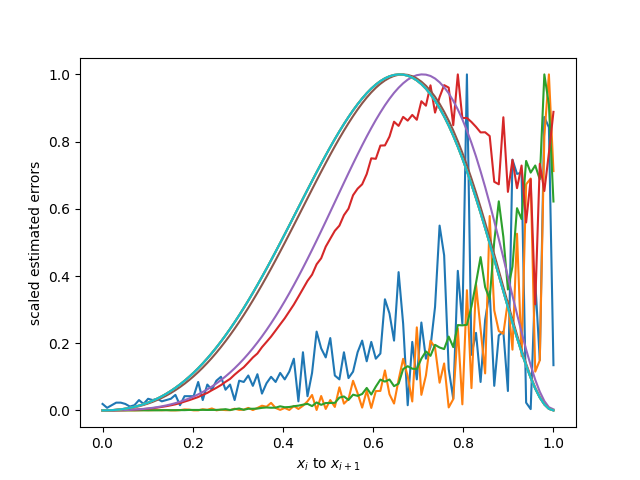
\includegraphics[width=0.7\linewidth]{./figures/rk8_with_hb8_hb10_sampling_p2_scaled_estimated_errors}
\caption{Scaled estimated errors over all steps for RK8 with HB8 vs HB10 with error sampling on problem 2 at an absolute tolerance of $10^{-6}$ mapped onto $[0, 1]$.}
\label{fig:rk8_with_hb8_hb10_sampling_p2_scaled_estimated_errors}
\end{figure}

\paragraph{Problem 3} Figures $\ref{fig:rk8_with_hb8_hb10_sampling_p3_global_error}$ and $\ref{fig:rk8_with_hb8_hb10_sampling_p3_scaled_errors}$ shows the global error and the shape of the error on each step of using rk8 with hb8 vs hb10 with sampling on Problem 3 at an absolute tolerance of $10^{-6}$. From Figure $\ref{fig:rk8_with_hb8_hb10_sampling_p3_scaled_errors}$, we can see that there is no consistent location where the exact error between the returned interpolant and the exact solution can be sampled. However, internally, the solver uses an estimated error between the two interpolants that it uses. In Figure $\ref{fig:rk8_with_hb8_hb10_sampling_p3_scaled_estimated_errors}$, we can see that the maximum error occurs reasonably consistently at $0.6h$.

\begin{figure}[H]
\centering
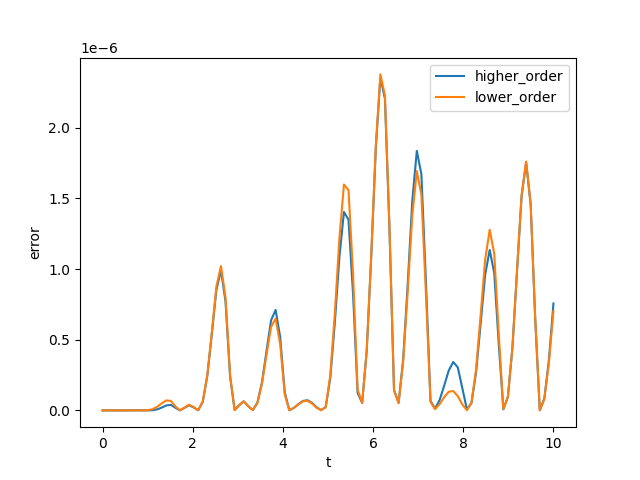
\includegraphics[width=0.7\linewidth]{./figures/rk8_with_hb8_hb10_sampling_p3_global_error}
\caption{Global Error for RK8 with HB8 vs HB10 with error sampling on problem 3 at an absolute tolerance of $10^{-6}$.}
\label{fig:rk8_with_hb8_hb10_sampling_p3_global_error}
\end{figure}

\begin{figure}[H]
\centering
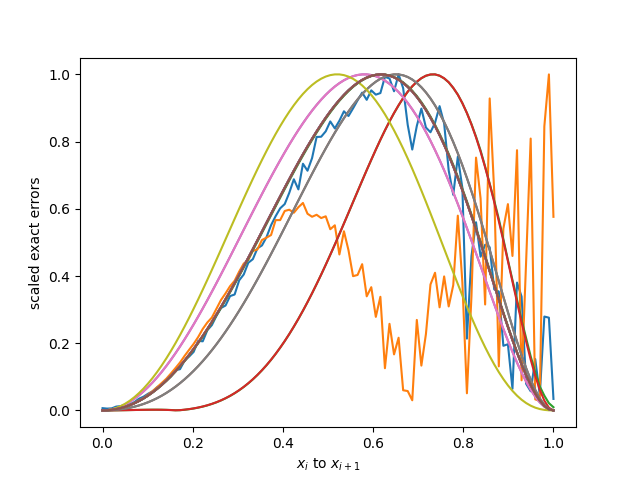
\includegraphics[width=0.7\linewidth]{./figures/rk8_with_hb8_hb10_sampling_p3_scaled_errors}
\caption{Scaled exact errors over all steps for RK8 with HB8 vs HB10 with error sampling on problem 3 at an absolute tolerance of $10^{-6}$ mapped onto $[0, 1]$.}
\label{fig:rk8_with_hb8_hb10_sampling_p3_scaled_errors}
\end{figure}

\begin{figure}[H]
\centering
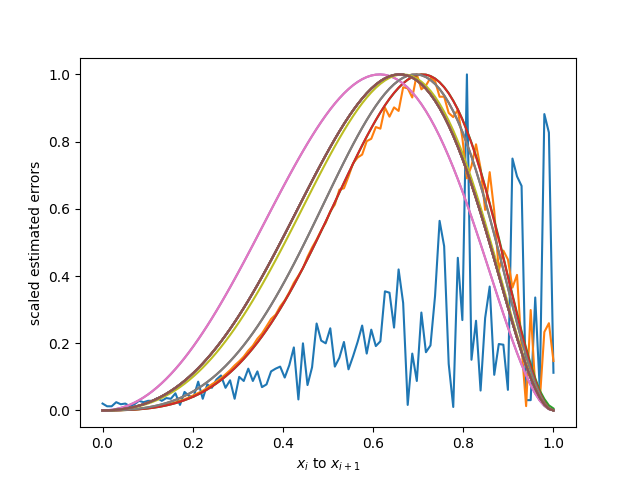
\includegraphics[width=0.7\linewidth]{./figures/rk8_with_hb8_hb10_sampling_p3_scaled_estimated_errors}
\caption{Scaled estimated errors over all steps for RK8 with HB8 vs HB10 with error sampling on problem 3 at an absolute tolerance of $10^{-6}$ mapped onto $[0, 1]$.}
\label{fig:rk8_with_hb8_hb10_sampling_p3_scaled_estimated_errors}
\end{figure}

\begin{table}[h]
\caption {Number of steps taken by RK8 using error control with HB8 vs HB10 by sampling the error.} \label{tab:rk8_with_hb8_hb10_sampling_nsteps}
\begin{center}
\begin{tabular}{ c c c } 
Problem & successful steps & total steps \\ 
1       & 14               & 16 \\ 
2       & 10               & 15 \\
3       & 16               & 24 \\
\end{tabular}
\end{center}
\end{table}

\subsection{comparison with crk65 and crk87 error sampling}
We also do continuous error sampling with crk65 and crk87 because both are equipped with a lower order interpolants and higher order interpolants. 

In this section we compare crk65 with rk6 with hb6 vs hb8 and compare crk87 with rk8 with hb8 vs hb10.

We use the same initial step size and same step selection algorithm as we did in both experiments. However we should note that all the solvers above can be optimised based on their respective theories.

\subsubsection{crk65 vs rk6 with hb6 vs hb8}

\paragraph{Problem 1} Figures $\ref{fig:crk65_sampling_p1_global_error}$ and $\ref{fig:crk65_sampling_p1_scaled_errors}$ shows the global error and the shape of the error on each step of using crk65 with sampling on Problem 1 at an absolute tolerance of $10^{-6}$. From Figure $\ref{fig:crk65_sampling_p1_scaled_errors}$, we can see that there is no consistent location where the exact error between the returned interpolant and the exact solution can be sampled. However, internally, the solver uses an estimated error between the two interpolants that it uses. In Figure $\ref{fig:crk65_sampling_p1_scaled_estimated_errors}$, we can see that the maximum error occurs reasonably consistently at $0.5h$.

\begin{figure}[H]
\centering
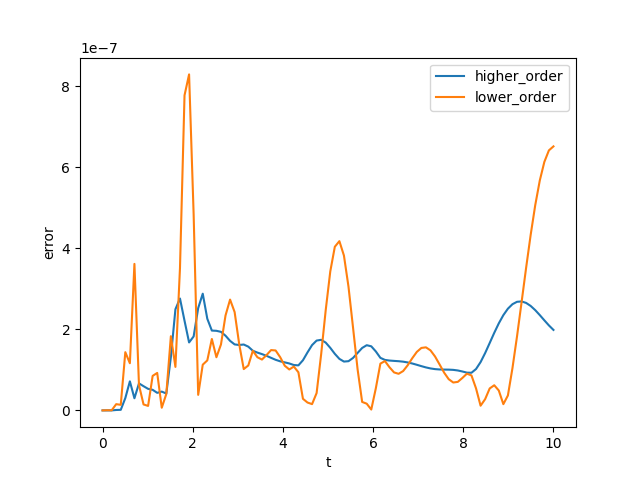
\includegraphics[width=0.7\linewidth]{./figures/crk65_sampling_p1_global_error}
\caption{Global Error for CRK65 with error sampling on problem 1 at an absolute tolerance of $10^{-6}$.}
\label{fig:crk65_sampling_p1_global_error}
\end{figure}

\begin{figure}[H]
\centering
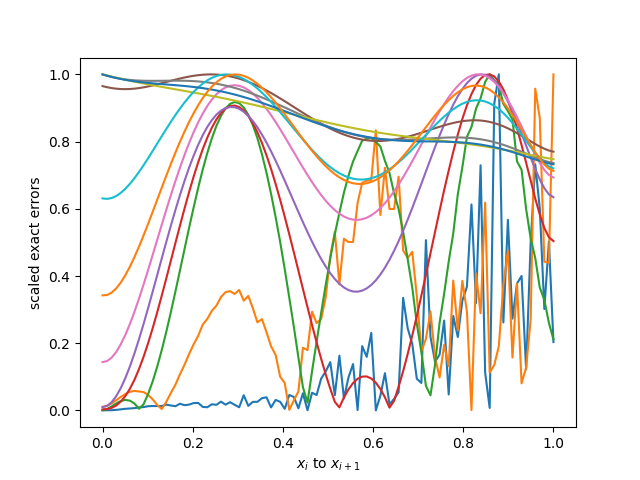
\includegraphics[width=0.7\linewidth]{./figures/crk65_sampling_p1_scaled_errors}
\caption{Scaled exact errors over all steps for CRK65 with error sampling on problem 1 at an absolute tolerance of $10^{-6}$ mapped onto $[0, 1]$.}
\label{fig:crk65_sampling_p1_scaled_errors}
\end{figure}

\begin{figure}[H]
\centering
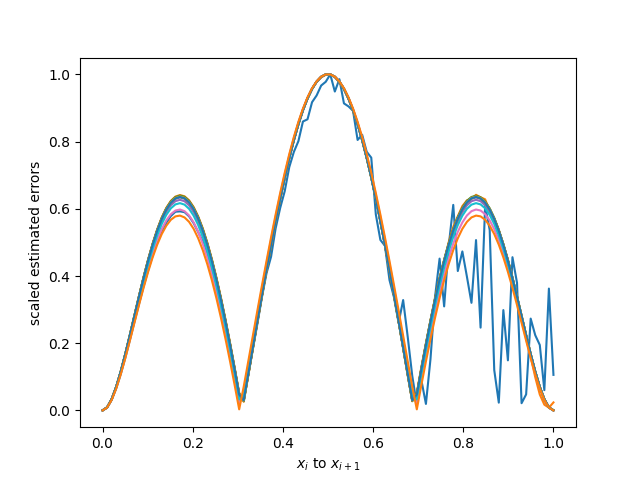
\includegraphics[width=0.7\linewidth]{./figures/crk65_sampling_p1_scaled_estimated_errors}
\caption{Scaled estimated errors over all steps for CRK65 with error sampling on problem 1 at an absolute tolerance of $10^{-6}$ mapped onto $[0, 1]$.}
\label{fig:crk65_sampling_p1_scaled_estimated_errors}
\end{figure}


\paragraph{Problem 2} Figures $\ref{fig:crk65_sampling_p2_global_error}$ and $\ref{fig:crk65_sampling_p2_scaled_errors}$ shows the global error and the shape of the error on each step of using crk65 with sampling on Problem 2 at an absolute tolerance of $10^{-6}$. From Figure $\ref{fig:crk65_sampling_p2_scaled_errors}$, we can see that there is no consistent location where the exact error between the returned interpolant and the exact solution can be sampled. However, internally, the solver uses an estimated error between the two interpolants that it uses. In Figure $\ref{fig:crk65_sampling_p2_scaled_estimated_errors}$, we can see that the maximum error occurs reasonably consistently at $0.6h$.

\begin{figure}[H]
\centering
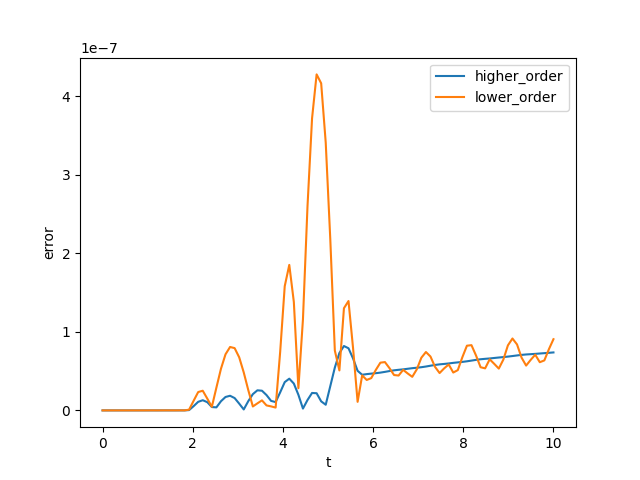
\includegraphics[width=0.7\linewidth]{./figures/crk65_sampling_p2_global_error}
\caption{Global Error for CRK65 with error sampling on problem 2 at an absolute tolerance of $10^{-6}$.}
\label{fig:crk65_sampling_p2_global_error}
\end{figure}

\begin{figure}[H]
\centering
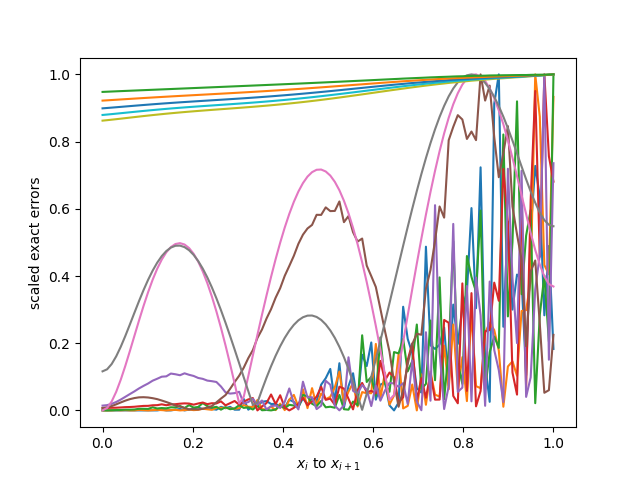
\includegraphics[width=0.7\linewidth]{./figures/crk65_sampling_p2_scaled_errors}
\caption{Scaled exact errors over all steps for CRK65 with error sampling on problem 2 at an absolute tolerance of $10^{-6}$ mapped onto $[0, 1]$.}
\label{fig:crk65_sampling_p2_scaled_errors}
\end{figure}

\begin{figure}[H]
\centering
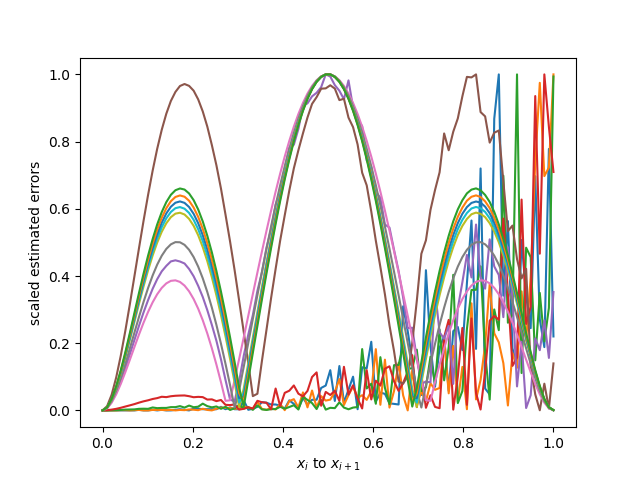
\includegraphics[width=0.7\linewidth]{./figures/crk65_sampling_p2_scaled_estimated_errors}
\caption{Scaled estimated errors over all steps for CRK65 with error sampling on problem 2 at an absolute tolerance of $10^{-6}$ mapped onto $[0, 1]$.}
\label{fig:crk65_sampling_p2_scaled_estimated_errors}
\end{figure}

\paragraph{Problem 3} Figures $\ref{fig:crk65_sampling_p3_global_error}$ and $\ref{fig:crk65_sampling_p3_scaled_errors}$ shows the global error and the shape of the error on each step of using crk65 with sampling on Problem 3 at an absolute tolerance of $10^{-6}$. From Figure $\ref{fig:crk65_sampling_p3_scaled_errors}$, we can see that there is no consistent location where the exact error between the returned interpolant and the exact solution can be sampled. However, internally, the solver uses an estimated error between the two interpolants that it uses. In Figure $\ref{fig:crk65_sampling_p3_scaled_estimated_errors}$, we can see that the maximum error occurs reasonably consistently at $0.6h$.

\begin{figure}[H]
\centering
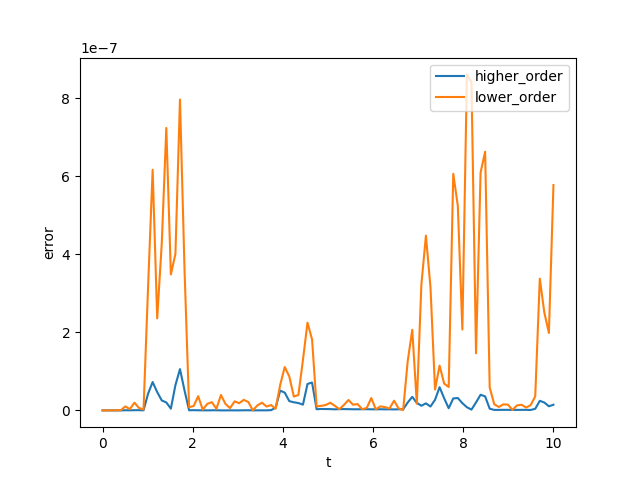
\includegraphics[width=0.7\linewidth]{./figures/crk65_sampling_p3_global_error}
\caption{Global Error for CRK65 with error sampling on problem 3 at an absolute tolerance of $10^{-6}$.}
\label{fig:crk65_sampling_p3_global_error}
\end{figure}

\begin{figure}[H]
\centering
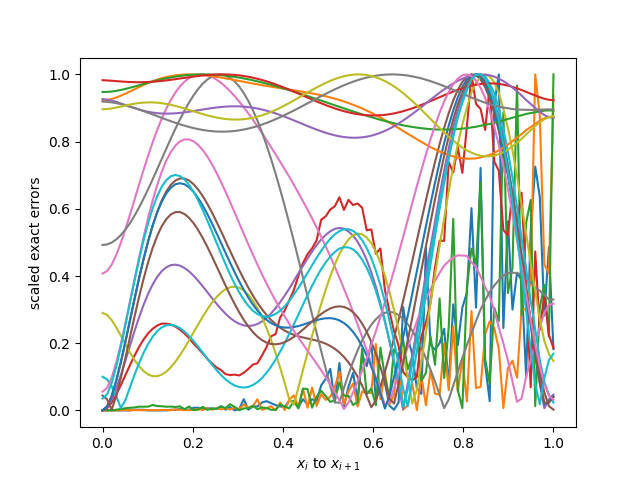
\includegraphics[width=0.7\linewidth]{./figures/crk65_sampling_p3_scaled_errors}
\caption{Scaled exact errors over all steps for CRK65 with error sampling on problem 3 at an absolute tolerance of $10^{-6}$ mapped onto $[0, 1]$.}
\label{fig:crk65_sampling_p3_scaled_errors}
\end{figure}

\begin{figure}[H]
\centering
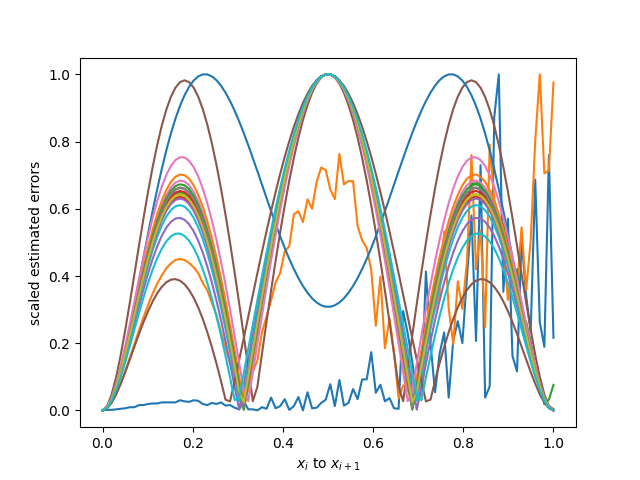
\includegraphics[width=0.7\linewidth]{./figures/crk65_sampling_p3_scaled_estimated_errors}
\caption{Scaled estimated errors over all steps for CRK65 with error sampling on problem 3 at an absolute tolerance of $10^{-6}$ mapped onto $[0, 1]$.}
\label{fig:crk65_sampling_p3_scaled_estimated_errors}
\end{figure}

\begin{table}[h]
\caption {Number of steps taken by CRK65 using error control with error sampling its two interpolants.} \label{tab:crk65_sampling_nsteps}
\begin{center}
\begin{tabular}{ c c c } 
Problem & successful steps & total steps \\ 
1       & 12               & 12 \\ 
2       & 13               & 19 \\
3       & 20               & 30 \\
\end{tabular}
\end{center}
\end{table}

Comparing Table $\ref{tab:rk6_with_hb6_hb8_sampling_nsteps}$ and Table $\ref{tab:crk65_sampling_nstep}$, we can see that we can get similar number of steps without paying for additional stages. We can also see that we get similar levels of accuracy.

\subsubsection{crk87 vs rk8 with hb8 vs hb10}

\paragraph{Problem 1} Figures $\ref{fig:crk87_sampling_p1_global_error}$ and $\ref{fig:crk87_sampling_p1_scaled_errors}$ shows the global error and the shape of the error on each step of using crk87 with sampling on Problem 1 at an absolute tolerance of $10^{-6}$. From Figure $\ref{fig:crk87_sampling_p1_scaled_errors}$, we can see that there is no consistent location where the exact error between the returned interpolant and the exact solution can be sampled. However, internally, the solver uses an estimated error between the two interpolants that it uses. In Figure $\ref{fig:crk87_sampling_p1_scaled_estimated_errors}$, we can see that the maximum error occurs reasonably consistently at $0.5h$. CONSISTENT MAXIMUM IS NOT THE CASE FOR crk87 =============================================

\begin{figure}[H]
\centering
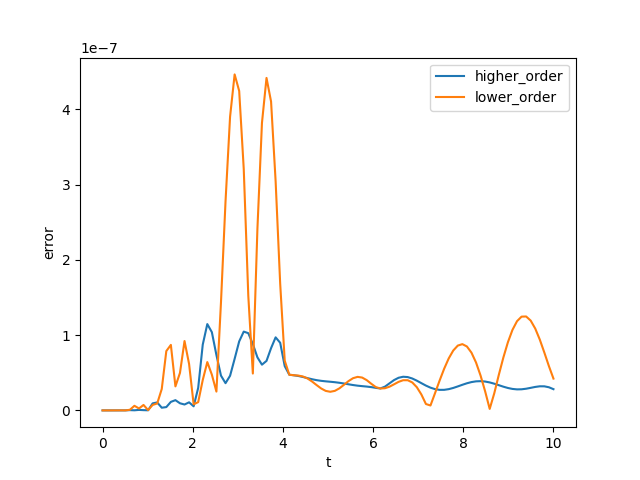
\includegraphics[width=0.7\linewidth]{./figures/crk87_sampling_p1_global_error}
\caption{Global Error for CRK87 with error sampling on problem 1 at an absolute tolerance of $10^{-6}$.}
\label{fig:crk87_sampling_p1_global_error}
\end{figure}

\begin{figure}[H]
\centering
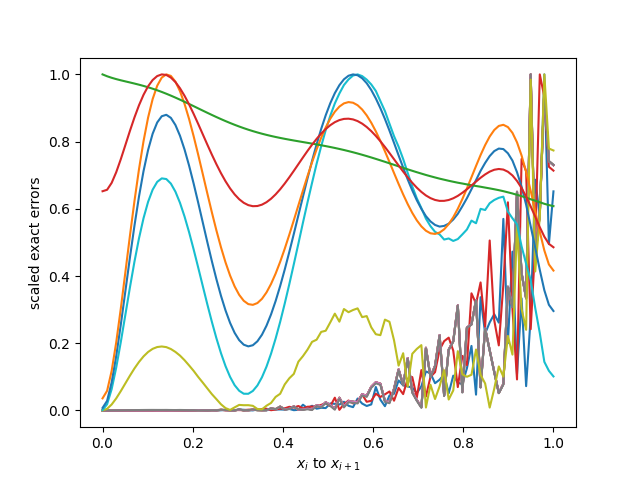
\includegraphics[width=0.7\linewidth]{./figures/crk87_sampling_p1_scaled_errors}
\caption{Scaled exact errors over all steps for CRK87 with error sampling on problem 1 at an absolute tolerance of $10^{-6}$ mapped onto $[0, 1]$.}
\label{fig:crk87_sampling_p1_scaled_errors}
\end{figure}

\begin{figure}[H]
\centering
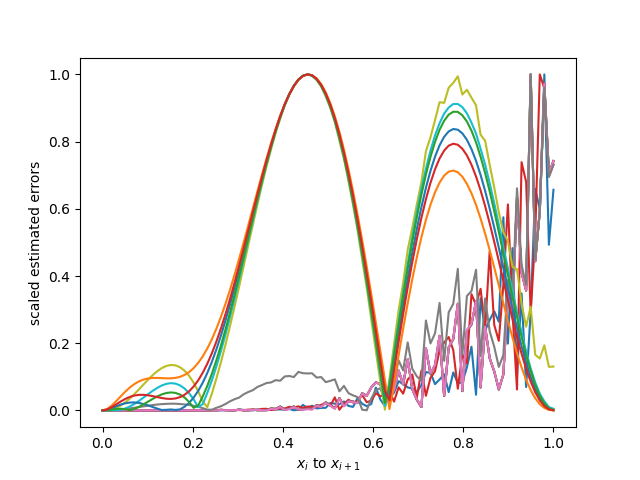
\includegraphics[width=0.7\linewidth]{./figures/crk87_sampling_p1_scaled_estimated_errors}
\caption{Scaled estimated errors over all steps for CRK87 with error sampling on problem 1 at an absolute tolerance of $10^{-6}$ mapped onto $[0, 1]$.}
\label{fig:crk87_sampling_p1_scaled_estimated_errors}
\end{figure}


\paragraph{Problem 2} Figures $\ref{fig:crk87_sampling_p2_global_error}$ and $\ref{fig:crk87_sampling_p2_scaled_errors}$ shows the global error and the shape of the error on each step of using crk87 with sampling on Problem 2 at an absolute tolerance of $10^{-6}$. From Figure $\ref{fig:crk87_sampling_p2_scaled_errors}$, we can see that there is no consistent location where the exact error between the returned interpolant and the exact solution can be sampled. However, internally, the solver uses an estimated error between the two interpolants that it uses. In Figure $\ref{fig:crk87_sampling_p2_scaled_estimated_errors}$, we can see that the maximum error occurs reasonably consistently at $0.6h$.  CONSISTENT MAXIMUM IS NOT THE CASE FOR crk87 =============================================

\begin{figure}[H]
\centering
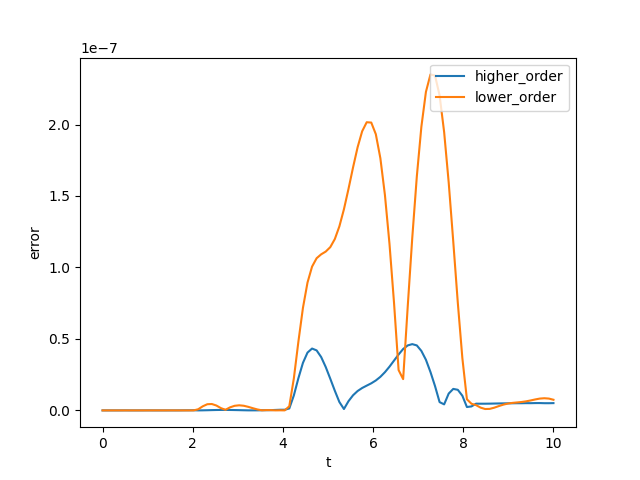
\includegraphics[width=0.7\linewidth]{./figures/crk87_sampling_p2_global_error}
\caption{Global Error for CRK87 with error sampling on problem 2 at an absolute tolerance of $10^{-6}$.}
\label{fig:crk87_sampling_p2_global_error}
\end{figure}

\begin{figure}[H]
\centering
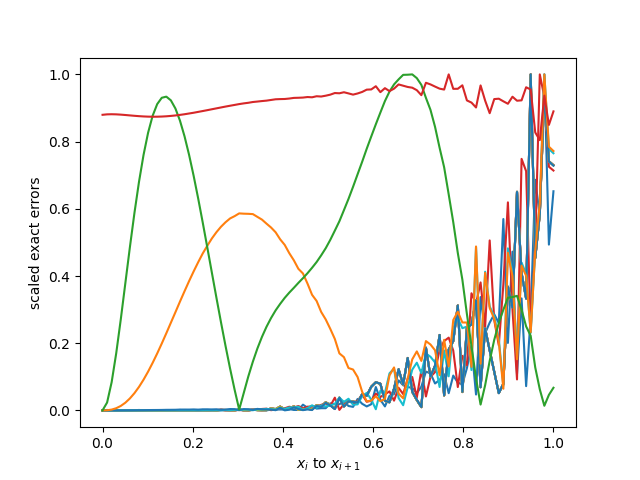
\includegraphics[width=0.7\linewidth]{./figures/crk87_sampling_p2_scaled_errors}
\caption{Scaled exact errors over all steps for CRK87 with error sampling on problem 2 at an absolute tolerance of $10^{-6}$ mapped onto $[0, 1]$.}
\label{fig:crk87_sampling_p2_scaled_errors}
\end{figure}

\begin{figure}[H]
\centering
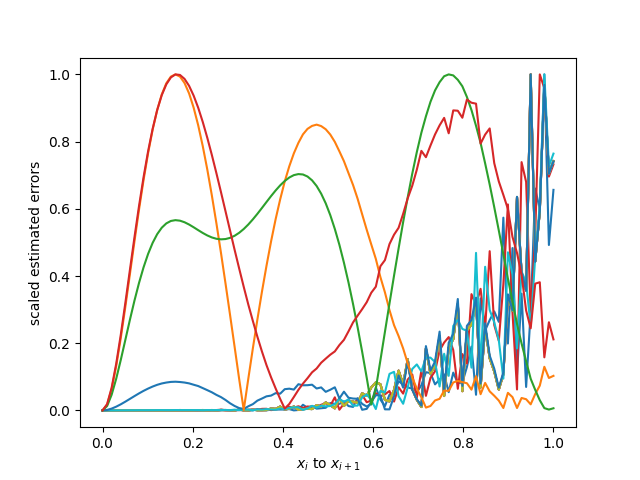
\includegraphics[width=0.7\linewidth]{./figures/crk87_sampling_p2_scaled_estimated_errors}
\caption{Scaled estimated errors over all steps for CRK87 with error sampling on problem 2 at an absolute tolerance of $10^{-6}$ mapped onto $[0, 1]$.}
\label{fig:crk87_sampling_p2_scaled_estimated_errors}
\end{figure}

\paragraph{Problem 3} Figures $\ref{fig:crk87_sampling_p3_global_error}$ and $\ref{fig:crk87_sampling_p3_scaled_errors}$ shows the global error and the shape of the error on each step of using crk87 with sampling on Problem 3 at an absolute tolerance of $10^{-6}$. From Figure $\ref{fig:crk87_sampling_p3_scaled_errors}$, we can see that there is no consistent location where the exact error between the returned interpolant and the exact solution can be sampled. However, internally, the solver uses an estimated error between the two interpolants that it uses. In Figure $\ref{fig:crk87_sampling_p3_scaled_estimated_errors}$, we can see that the maximum error occurs reasonably consistently at $0.6h$.  CONSISTENT MAXIMUM IS NOT THE CASE FOR crk87 =============================================

\begin{figure}[H]
\centering
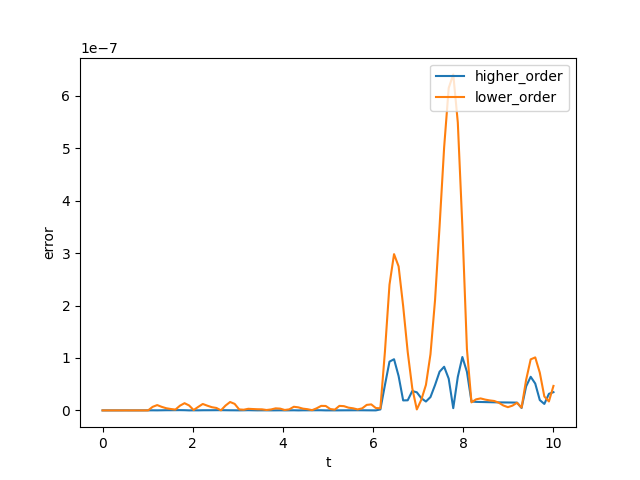
\includegraphics[width=0.7\linewidth]{./figures/crk87_sampling_p3_global_error}
\caption{Global Error for CRK87 with error sampling on problem 3 at an absolute tolerance of $10^{-6}$.}
\label{fig:crk87_sampling_p3_global_error}
\end{figure}

\begin{figure}[H]
\centering
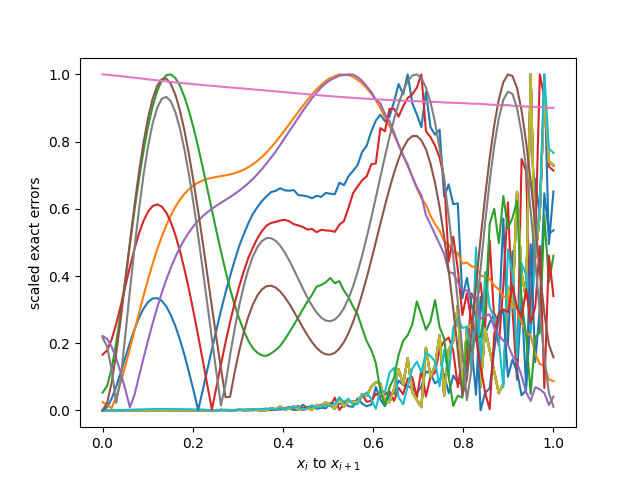
\includegraphics[width=0.7\linewidth]{./figures/crk87_sampling_p3_scaled_errors}
\caption{Scaled exact errors over all steps for CRK87 with error sampling on problem 3 at an absolute tolerance of $10^{-6}$ mapped onto $[0, 1]$.}
\label{fig:crk87_sampling_p3_scaled_errors}
\end{figure}

\begin{figure}[H]
\centering
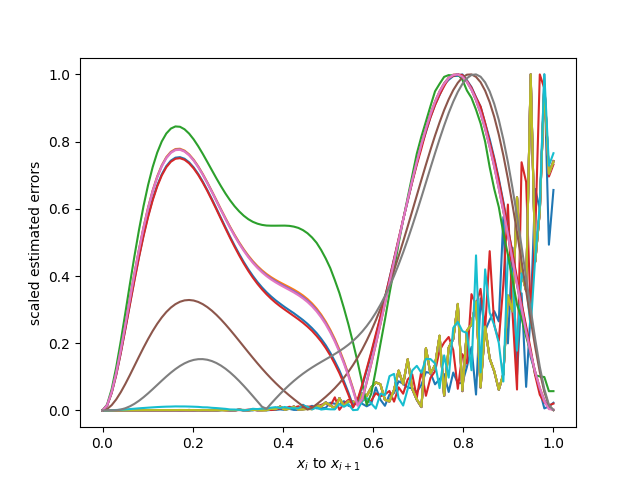
\includegraphics[width=0.7\linewidth]{./figures/crk87_sampling_p3_scaled_estimated_errors}
\caption{Scaled estimated errors over all steps for CRK87 with error sampling on problem 3 at an absolute tolerance of $10^{-6}$ mapped onto $[0, 1]$.}
\label{fig:crk87_sampling_p3_scaled_estimated_errors}
\end{figure}

\begin{table}[h]
\caption {Number of steps taken by CRK87 using error control with error sampling its two interpolants.} \label{tab:crk87_sampling_nsteps}
\begin{center}
\begin{tabular}{ c c c } 
Problem & successful steps & total steps \\ 
1       & 8               & 8 \\ 
2       & 8               & 10 \\
3       & 10              & 12 \\
\end{tabular}
\end{center}
\end{table}

Table $\ref{tab:rk8_with_hb8_hb10_sampling_nsteps}$ and $\ref{tab:crk87_sampling_nsteps}$ shows the number of steps for crk87 are not too close to rk8 with hb8 vs hb10 but close enough. WE also note that rk8 with hb8 vs hb10 is two times less expensive.

 